\documentclass[11pt,twocolumn]{article}
\usepackage[margin=0.76in]{geometry}
\usepackage{amsmath,amssymb,amsthm}
\usepackage{booktabs}
\usepackage{graphicx}
\usepackage{hyperref}
\usepackage{xcolor}

\newtheorem{proposition}{Proposition}
\newtheorem{remark}{Remark}

\title{\textbf{Dual-Processor Certification of Schmidt Number $\ge 3$ and $>1$-Ebit Entanglement of Formation in Hayden--Preskill Recovery via Layout-Locked Nine-Basis Stabilizer Tomography on Heavy-Hex Superconducting Processors}}

\author{Devin Phillip Davis\\
\small Agile Defense Systems LLC\\
\small Pre-Registered Benchmarks \texttt{OSIRIS-HP-004} (\texttt{ibm\_marrakesh} Job \texttt{dbti1fbsbsbs73cb2vu0}) \& \texttt{OSIRIS-HP-004B} (\texttt{ibm\_fez} Job \texttt{dbtj61bnlcms73ajc380})\\
\small Version 2.1 (Adds Primary Terhal--Vollbrecht Citation, Exact $F_* = 0.683900$ Root, and Legacy JSON Schema Note; v2.0 Frozen at \texttt{10.5281/zenodo.24287505})}

\date{November 16, 2026}

\begin{document}
\maketitle

\begin{abstract}
Experimental realizations of multi-qubit Hayden--Preskill information recovery on noisy superconducting processors face three distinct pitfalls: (i) measuring two-qubit marginal fidelities in only three global Pauli bases ($XX, YY, ZZ$) cannot rule out a Schmidt-number-$2$ mixture achieving marginal fidelity $\bar{F}=0.7500$ and product $F_1 F_2 = 0.5625$ while possessing four-qubit joint overlap $F_{\mathrm{joint}}=0.5000$; (ii) unconstrained hardware compilation can insert hidden routing SWAPs across quarantined horizon subsystems; and (iii) exceeding the $F_{\mathrm{joint}}=0.5000$ Schmidt-number-$2$ ceiling~\cite{TerhalHorodecki2000} certifies entanglement dimensionality $\mathrm{SN}(\rho)\ge 3$ (ruling out any rank-$\le 2$ / single-qubit quantum channel plus LOCC) rather than Entanglement of Formation $E_F(\rho)>1\text{ ebit}$, whose exact $d=4$ isotropic convex-roof threshold is $F_* = 0.683900$ ($0.683900317$)~\cite{TerhalVollbrecht2000,VollbrechtWerner2001}. Here we report two prospectively pre-registered, layout-locked $8$-qubit experiments across independent $156$-qubit IBM Heron r2 processors---\texttt{OSIRIS-HP-004} on \texttt{ibm\_marrakesh} (Job \texttt{dbti1fbsbsbs73cb2vu0}) and \texttt{OSIRIS-HP-004B} on \texttt{ibm\_fez} (Job \texttt{dbtj61bnlcms73ajc380})---totaling $572$ circuits $\times 1{,}024$ shots $= 585{,}728$ raw shots (\texttt{resilience\_level=0}, zero postselection). Embedding a $7$-CZ dual-unitary Clifford scrambler and an exact $10$-CZ symplectic restricted decoder onto isomorphic $8$-transmon heavy-hex trees with \texttt{routing\_method="none"}, reference leaves and horizon remnants experience zero physical gates during decoding. Measuring all nine two-pair Pauli settings $\{X,Y,Z\}_1\times\{X,Y,Z\}_2$ ($16$ Bell stabilizers), raw unmitigated restricted recovery (\texttt{Arm B}, $32$ CZs) achieves $F_{\mathrm{joint}}=0.6334 \pm 0.0026$ on \texttt{ibm\_marrakesh} ($+50.64\sigma$ above $0.5000$, certifying $\mathrm{SN}(\rho)\ge 3$ and $E_F(\rho)\ge 0.8451\text{ ebits}$, whereas $3$-basis marginals yield $F_1+F_2-1=0.4875<0.50$) and $F_{\mathrm{joint}}=0.7307 \pm 0.0027$ on \texttt{ibm\_fez} ($6$-block $95\%$ Student-$t$ CI $[0.7237, 0.7377]$, certifying \emph{both} $\mathrm{SN}(\rho)\ge 3$ at $+84.45\sigma$ and $E_F(\rho)\ge 1.1465 \pm 0.0086\text{ ebits} > 1\text{ ebit}$ at $+17.13\sigma$). Across both processors, all $10/10$ pre-registered hypotheses pass and resolve the full dyadic capacity ladder ($1/16, 2/16, 4/16, 8/16, 16/16$).
\end{abstract}

\section{Introduction and Witness Thresholds}
In the Hayden--Preskill protocol~\cite{HaydenPreskill2007}, a $k$-qubit system entangled with an isolated reference $R$ enters an $n$-qubit scrambler $B$ maximally entangled with early radiation $E$. When scrambling decouples $R$ from the surviving horizon remnant $C$ ($I(R:C)=0$), coherent decoding on $E$ together with $k_D\ge k$ late radiation qubits $D$ recovers the joint state with $R$~\cite{YoshidaKitaev2017,Landsman2019}.

Scaling from $k=1$ ($6$ qubits) to $k=2$ ($8$ qubits: $R_1,R_2,M_1,M_2,B_1,B_2,E_1,E_2$) requires distinguishing two inequivalent operational thresholds on the recovered $4\times 4$ state $\rho$ across $(R_2 R_1):(M_1' M_2')$, with target $|\Psi_4\rangle = |\Phi^+\rangle_{R_2 M_1'}\otimes|\Phi^+\rangle_{R_1 M_2'}$:

\begin{proposition}[Schmidt-Number-2 Witness~\cite{TerhalHorodecki2000}]
For every $4$-qubit mixed state $\rho$ across $(R_2 R_1):(M_1' M_2')$ of Schmidt number $\mathrm{SN}(\rho)\le 2$ (including any state transmissible via a single noiseless qubit channel or one shared $2\times 2$ Bell pair plus LOCC),
\begin{equation}
F_{\mathrm{joint}}(\rho) \equiv \langle \Psi_4|\rho|\Psi_4\rangle \le \frac{2}{4} = 0.5000.
\label{eq:sn2_bound}
\end{equation}
Conversely, the explicit $\mathrm{SN}=2$ classical mixture
\begin{align}
\rho_{\mathrm{SR2}} = \frac{1}{4}\Big(
&|\Phi^+\rangle_1\langle\Phi^+|\otimes |00\rangle_2\langle 00|
+ |\Phi^+\rangle_1\langle\Phi^+|\otimes |11\rangle_2\langle 11| \nonumber\\
+\,&|00\rangle_1\langle 00|\otimes |\Phi^+\rangle_2\langle\Phi^+|
+ |11\rangle_1\langle 11|\otimes |\Phi^+\rangle_2\langle\Phi^+| \Big)
\end{align}
achieves $2$-qubit marginals $F_1=F_2=\bar{F}=0.7500$ and $F_1 F_2 = 0.5625$ while saturating $F_{\mathrm{joint}}(\rho_{\mathrm{SR2}})=0.5000$.
\end{proposition}

\begin{proposition}[Entanglement of Formation Threshold~\cite{TerhalVollbrecht2000,VollbrechtWerner2001}]
Exceeding $F_{\mathrm{joint}}=0.5000$ certifies $\mathrm{SN}(\rho)\ge 3$ but does \emph{not} by itself establish Entanglement of Formation $E_F(\rho)>1\text{ ebit}$: for example, a pure state with Schmidt probabilities $(0.85, 0.05, 0.05, 0.05)$ has $F_{\mathrm{joint}}=\frac{1}{4}(\sqrt{0.85}+3\sqrt{0.05})^2 \approx 0.6342 > 0.5000$ yet entanglement entropy $H_2 = 0.8476\text{ ebits} < 1$. By the Terhal--Vollbrecht theorem for $d=4$ isotropic states~\cite{TerhalVollbrecht2000} and the Vollbrecht--Werner symmetry framework~\cite{VollbrechtWerner2001}, for $F_{\mathrm{joint}}\in[\frac{1}{4},\frac{3}{4}]$ the exact convex-roof lower bound is
\begin{equation}
E_F(\rho) \ge \gamma_4(F_{\mathrm{joint}}) = H_2\!\left(p_0, \tfrac{1-p_0}{3}, \tfrac{1-p_0}{3}, \tfrac{1-p_0}{3}\right),
\label{eq:ef_bound}
\end{equation}
where $p_0(F) = \frac{1}{4}(\sqrt{F}+\sqrt{3(1-F)})^2$ ($\gamma_4''(F)>0$ on $[\frac{1}{4},\frac{3}{4}]$). In particular, $\gamma_4(F_*) = 1.0000\text{ ebit}$ occurs at the unique root
\begin{equation}
F_* = 0.683900\quad (0.683900317\ldots).
\label{eq:fstar}
\end{equation}
\end{proposition}

\begin{remark}[Version 2.0 $\to$ 2.1 Revision and Schema Note]
Version~1.0 (\texttt{10.5281/zenodo.24285577}, reporting \texttt{ibm\_marrakesh} alone) loosely referred to $F_{\mathrm{joint}}>0.5000$ as certifying ``$>1\text{ ebit}$''; Version~2.0 (\texttt{10.5281/zenodo.24287505}) corrected that wording and added the \texttt{ibm\_fez} cross-processor replication ($0.7307$), which exceeds both $0.5000$ ($+84.45\sigma$) and $F_*=0.683900$ ($+17.13\sigma$; $E_F(\rho)\ge 1.1465 \pm 0.0086\text{ ebits}$, $95\%$ $t$-LCL $0.7237 \Rightarrow E_F \ge 1.1244\text{ ebits}$). Version~2.1 adds the primary isotropic-state $E_F$ reference~\cite{TerhalVollbrecht2000}, refines the fifth decimal of $F_*$ ($0.683910 \to 0.683900$), and records for downstream parsers of the frozen \texttt{Zenodo 24287505} JSON artifacts (\texttt{physical\_hp004*\_results.json}) that the legacy key \texttt{z\_above\_1ebit\_eff} computes $(F_{\mathrm{joint}}-0.5000)/\mathrm{SE}_{\mathrm{eff}}$ ($Z$ above the $0.5000$ $\mathrm{SN}\le 2$ ceiling: $+50.64$ on \texttt{ibm\_marrakesh}, $+84.45$ on \texttt{ibm\_fez}), whereas $Z$ above $F_* = 0.683900$ is $-19.16\sigma$ on \texttt{ibm\_marrakesh} and $+17.13\sigma$ on \texttt{ibm\_fez}. All bounds are witness-derived convex-roof lower bounds conditional on target-state mapping and faithful Pauli basis settings, not direct von Neumann entropy measurements.
\end{remark}

Reconstructing $F_{\mathrm{joint}}$ without factorization assumptions measures all $16$ stabilizers across all nine Pauli settings $(P,Q)\in\{X,Y,Z\}^2$:
\begin{equation}
F_{\mathrm{joint}} = \frac{1}{16}\!\left(1 + \sum_{P} s_P\langle P_1\rangle + \sum_{Q} s_Q\langle Q_2\rangle + \sum_{P,Q} s_P s_Q\langle P_1 Q_2\rangle\right)\!,
\label{eq:fjoint}
\end{equation}
with $P_1 = P_{R_2}P_{M_1'}$, $Q_2 = Q_{R_1}Q_{M_2'}$, and $(s_X, s_Y, s_Z) = (+1, -1, +1)$.

\begin{figure}[t]
\centering
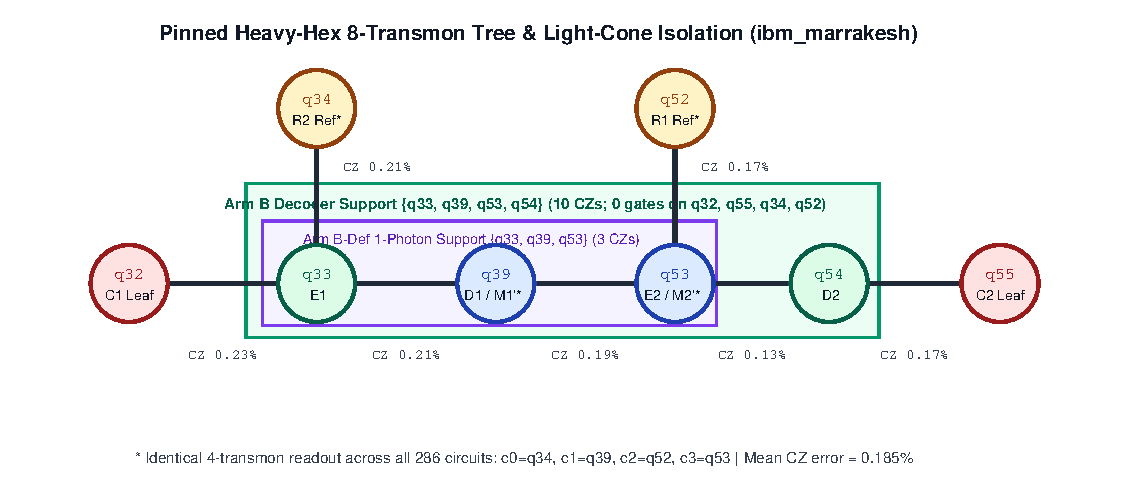
\includegraphics[width=\columnwidth]{fig3_marrakesh_tree_light_cone.pdf}\\[4pt]
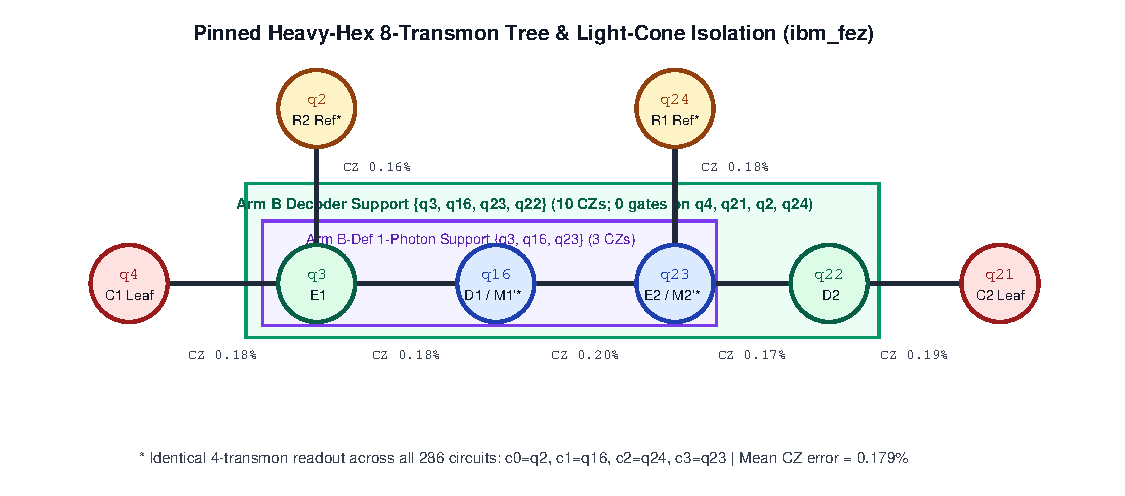
\includegraphics[width=\columnwidth]{fig4_fez_tree_light_cone.pdf}
\caption{Isomorphic $8$-transmon heavy-hex trees pinned with \texttt{routing\_method="none"} on \texttt{ibm\_marrakesh} (top, mean CZ error $0.185\%$) and \texttt{ibm\_fez} (bottom, mean CZ error $0.179\%$). Reference leaves and outer horizon remnants sit strictly outside the $4$-transmon decoding support of \texttt{Arm B}.}
\label{fig:trees}
\end{figure}

\section{Isomorphic Heavy-Hex Tree Protocol}
We embed the $8$ logical subsystems $(w_0,\dots,w_7)=(R_2,R_1,C_1,E_1,D_1,E_2,D_2,C_2)$ onto isomorphic $8$-transmon heavy-hex trees on two distinct cryostats (Fig.~\ref{fig:trees}):
\begin{align*}
\texttt{ibm\_marrakesh}:&\; (34, 52, 32, 33, 39, 53, 54, 55),\\
\texttt{ibm\_fez}:&\; (2, 24, 4, 3, 16, 23, 22, 21).
\end{align*}
All $286$ circuits per processor are compiled with \texttt{routing\_method="none"}, validated via \texttt{validate\_isa\_circuits}, and locked to read out $(w_0, w_4, w_1, w_5) \to (c_0, c_1, c_2, c_3)$. Stage~1 ($6$ CZs; $4$ CZs in \texttt{Arm B-Ctrl}) prepares $|\Phi^+\rangle_{R_2 M_1}$, $|\Phi^+\rangle_{R_1 M_2}$, and early radiation $|\Phi^+\rangle_{B_1 E_1}\otimes|\Phi^+\rangle_{B_2 E_2}$, leaving $w_0, w_1$ idle thereafter. Stage~2 ($16$ CZs for $U_1$; $19$ CZs for $U_2$) applies a $7$-CZ dual-unitary Clifford scrambler ($I(R:D)=I(R:C)=I(R:E)=0$, $I(R:DE)=4\text{ bits}$) and routes remnants to outer tips $(w_2, w_7)$. Stage~3 compares five arms: barriered full unitary inverse \texttt{Arm A} ($38$ CZs); restricted $4$-qubit symplectic recovery \texttt{Arm B} ($32$ CZs on $\{w_3,w_4,w_5,w_6\}$, zero gates on $w_2, w_7$); unentangled $|0000\rangle_{BE}$ control \texttt{Arm B-Ctrl} ($30$ CZs); single-photon quarantined recovery \texttt{Arm B-Def} ($25$ CZs on $\{w_3,w_4,w_5\}$); and mismatched-scrambler control \texttt{Arm B-Held} ($35$ CZs).

\begin{figure}[t]
\centering
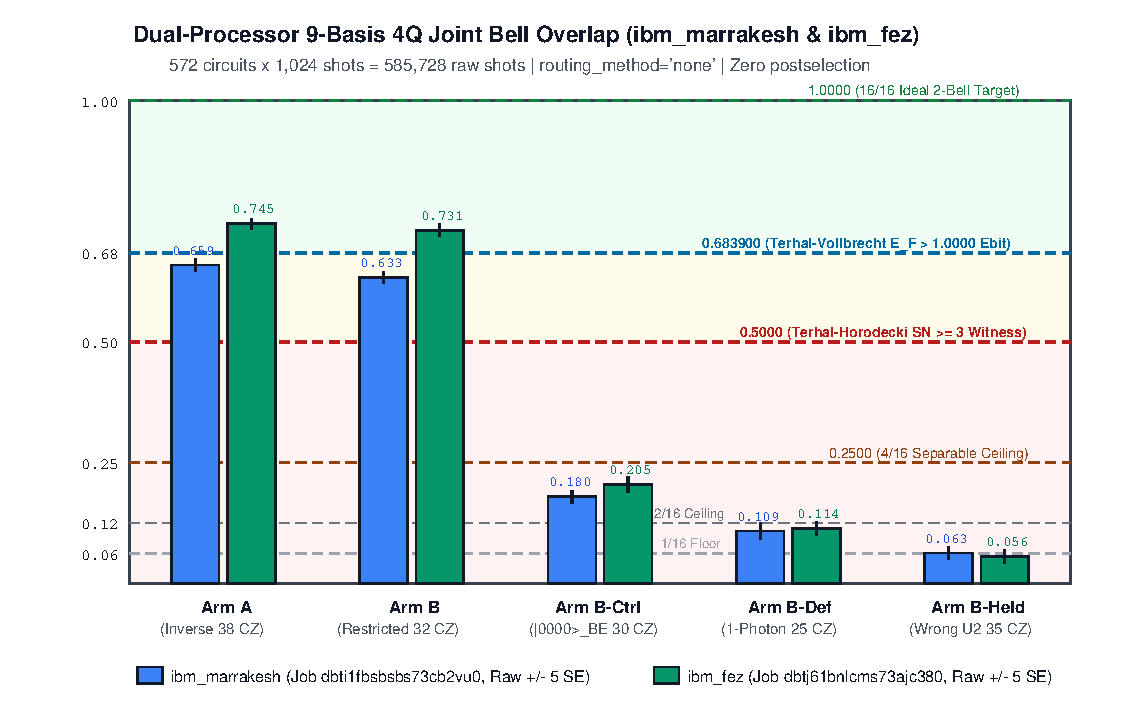
\includegraphics[width=\columnwidth]{fig1_dyadic_capacity_ladder.pdf}
\caption{Dual-processor $9$-basis joint Bell overlap $F_{\mathrm{joint}}$ across all five arms on \texttt{ibm\_marrakesh} (Job \texttt{dbti1fbsbsbs73cb2vu0}) and \texttt{ibm\_fez} (Job \texttt{dbtj61bnlcms73ajc380}; $585{,}728$ combined raw shots). Horizontal dashed lines denote the dyadic ladder ($1/16, 2/16, 4/16, 8/16$) and the Terhal--Vollbrecht $E_F>1\text{ ebit}$ threshold $F_*=0.683900$~\cite{TerhalVollbrecht2000,VollbrechtWerner2001}.}
\label{fig:ladder}
\end{figure}

\begin{table*}[t]
\centering
\caption{Prospectively pre-registered physical hardware measurements across \texttt{ibm\_marrakesh} (\texttt{OSIRIS-HP-004}, Job \texttt{dbti1fbsbsbs73cb2vu0}, $81\,\text{s}$ QPU) and \texttt{ibm\_fez} (\texttt{OSIRIS-HP-004B}, Job \texttt{dbtj61bnlcms73ajc380}, $79\,\text{s}$ QPU). Each job comprises $16$ SPAM circuits plus $6$ randomized blocks $\times$ $5$ arms $\times$ $9$ bases $\times$ $1{,}024$ shots ($292{,}864$ shots/processor; $\mathrm{SE}_{\mathrm{eff}}=\max(\mathrm{SEM}_{\mathrm{block,ddof=1}},\sigma_{\mathrm{shot}})$).}
\label{tab:results}
\footnotesize
\begin{tabular}{@{}llcccccccc@{}}
\toprule
\textbf{Processor} & \textbf{Arm (CZs)} & \textbf{Raw $F_1 \pm \sigma$} & \textbf{Raw $F_2 \pm \sigma$} & \textbf{Union $F_1\!+\!F_2\!-\!1$} & \textbf{Raw $F_{\mathrm{joint}} \pm \mathrm{SE}_{\mathrm{eff}}$} & \textbf{95\% Boot CI} & \textbf{$Z_{\mathrm{eff}}$ vs.\ $0.50$} & \textbf{$E_F$ Bound (ebits)} & \textbf{SPAM-Sec} \\
\midrule
\texttt{ibm\_marrakesh} & \texttt{Arm A} (38) & $0.7516 \pm 0.0024$ & $0.8006 \pm 0.0022$ & $+0.5522$ & $\mathbf{0.6591 \pm 0.0026}$ & $[0.6543, 0.6642]$ & $+61.67\sigma$ & $\ge 0.9235$ & $0.7194$ \\
\texttt{ibm\_marrakesh} & \texttt{Arm B} (32) & $0.7225 \pm 0.0025$ & $0.7650 \pm 0.0023$ & $+0.4875$ & $\mathbf{0.6334 \pm 0.0026}$ & $[0.6284, 0.6385]$ & $\mathbf{+50.64\sigma}$ & $\ge 0.8451$ & $0.6921$ \\
\texttt{ibm\_marrakesh} & \texttt{B-Ctrl} (30) & $0.4274 \pm 0.0029$ & $0.2476 \pm 0.0032$ & $-0.3250$ & $\mathbf{0.1799 \pm 0.0027}$ & $[0.1743, 0.1852]$ & $-117.03\sigma$ & $0$ & $0.1930$ \\
\texttt{ibm\_marrakesh} & \texttt{B-Def} (25) & $0.4174 \pm 0.0029$ & $0.2575 \pm 0.0032$ & $-0.3251$ & $\mathbf{0.1086 \pm 0.0035}$ & $[0.1032, 0.1142]$ & $-112.84\sigma$ & $0$ & $0.1123$ \\
\texttt{ibm\_marrakesh} & \texttt{B-Held} (35) & $0.2520 \pm 0.0032$ & $0.2560 \pm 0.0032$ & $-0.4920$ & $\mathbf{0.0634 \pm 0.0027}$ & $[0.0583, 0.0688]$ & $-164.67\sigma$ & $0$ & $0.0632$ \\
\midrule
\texttt{ibm\_fez} & \texttt{Arm A} (38) & $0.8174 \pm 0.0021$ & $0.8422 \pm 0.0020$ & $+0.6596$ & $\mathbf{0.7445 \pm 0.0023}$ & $[0.7400, 0.7491]$ & $+105.62\sigma$ & $\mathbf{\ge 1.1902}$ & $0.7755$ \\
\texttt{ibm\_fez} & \texttt{Arm B} (32) & $0.8124 \pm 0.0021$ & $0.8213 \pm 0.0021$ & $\mathbf{+0.6337}$ & $\mathbf{0.7307 \pm 0.0027}$ & $[0.7261, 0.7353]$ & $\mathbf{+84.45\sigma}$ & $\mathbf{\ge 1.1465}$ & $0.7611$ \\
\texttt{ibm\_fez} & \texttt{B-Ctrl} (30) & $0.4488 \pm 0.0028$ & $0.2554 \pm 0.0032$ & $-0.2958$ & $\mathbf{0.2053 \pm 0.0034}$ & $[0.2000, 0.2106]$ & $-87.78\sigma$ & $0$ & $0.2127$ \\
\texttt{ibm\_fez} & \texttt{B-Def} (25) & $0.4428 \pm 0.0029$ & $0.2516 \pm 0.0032$ & $-0.3056$ & $\mathbf{0.1140 \pm 0.0028}$ & $[0.1087, 0.1195]$ & $-137.72\sigma$ & $0$ & $0.1162$ \\
\texttt{ibm\_fez} & \texttt{B-Held} (35) & $0.2438 \pm 0.0032$ & $0.2511 \pm 0.0032$ & $-0.5051$ & $\mathbf{0.0563 \pm 0.0028}$ & $[0.0510, 0.0614]$ & $-158.96\sigma$ & $0$ & $0.0561$ \\
\bottomrule
\end{tabular}
\end{table*}

\begin{figure}[t]
\centering
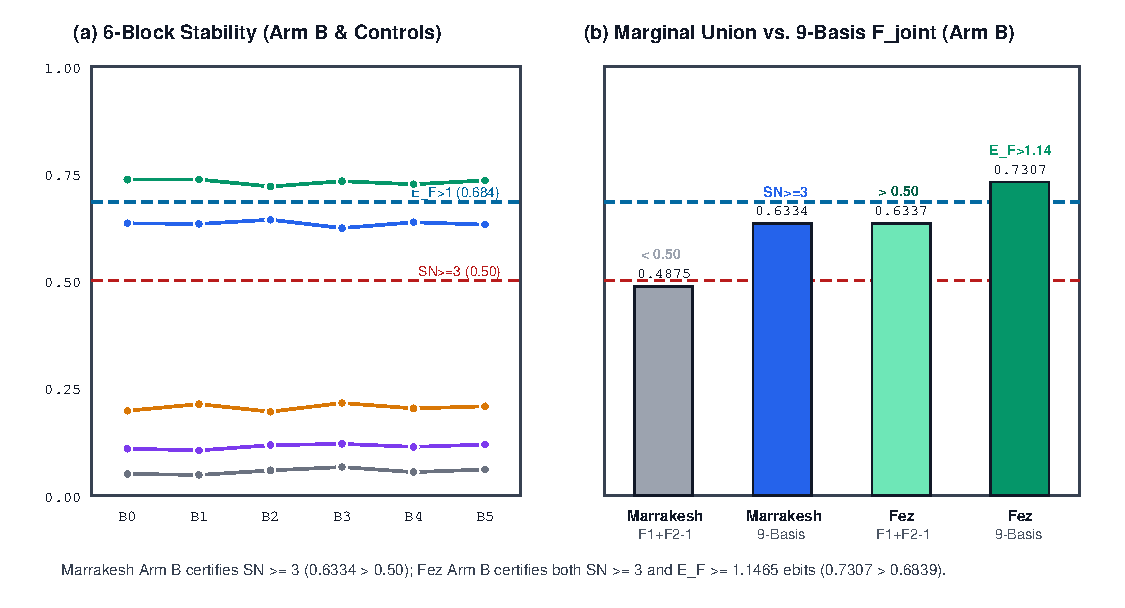
\includegraphics[width=\columnwidth]{fig2_block_stability_and_marginals.pdf}
\caption{(a) Six-block temporal stability of raw $F_{\mathrm{joint}}$ across \texttt{ibm\_fez} and \texttt{ibm\_marrakesh}. (b) Marginal union lower bound $F_1+F_2-1$ vs.\ $9$-basis $F_{\mathrm{joint}}$: on \texttt{ibm\_marrakesh}, $3$-basis marginals fall below $0.50$ ($0.4875$), whereas on lower-noise \texttt{ibm\_fez} ($97.31\%$ 4Q readout diagonal) both the marginal union bound ($0.6337$) and $9$-basis $F_{\mathrm{joint}}$ ($0.7307 > F_* = 0.683900$) cross their respective thresholds.}
\label{fig:blocks}
\end{figure}

\section{Dual-Processor Pre-Registration and Results}
Both runs were frozen and committed to GitHub prior to job creation: \texttt{fa9ef46d} (\texttt{15:26:18Z} $<$ \texttt{15:26:53Z}, QPY SHA-256 \texttt{c3daaa48d89a74ce...}) for \texttt{ibm\_marrakesh}, and \texttt{0c5a5a39} (\texttt{16:01:38Z} $<$ \texttt{16:44:53Z}, QPY SHA-256 \texttt{6d7e5a6d17a002b5...}) for \texttt{ibm\_fez}. Table~\ref{tab:results} and Figs.~\ref{fig:ladder}--\ref{fig:blocks} demonstrate three principal findings:
\begin{enumerate}
\item \textbf{Cross-Processor Replication of $\mathrm{SN}(\rho)\ge 3$ and $>1$-Ebit $E_F$:} On \texttt{ibm\_marrakesh}, raw \texttt{Arm B} ($0.6334 \pm 0.0026$; $6$-block $95\%$ $t$-CI $[0.6267, 0.6402]$) clears $0.5000$ by $+50.64\sigma$, certifying $\mathrm{SN}(\rho)\ge 3$ ($E_F \ge 0.8451\text{ ebits}$). On \texttt{ibm\_fez}, improved coupler ($0.179\%$ mean CZ) and readout ($97.31\%$ vs.\ $93.98\%$ 4Q diagonal) fidelities lift raw \texttt{Arm B} by $+0.0973$ to $0.7307 \pm 0.0027$ ($6$-block $95\%$ $t$-CI $[0.7237, 0.7377]$), clearing $0.5000$ by $+84.45\sigma$ \emph{and} clearing $F_*=0.683900$ by $+17.13\sigma$ ($E_F(\rho)\ge 1.1465 \pm 0.0086\text{ ebits}$; $95\%$ $t$-LCL bound $E_F \ge 1.1244\text{ ebits}$; $5\sigma$ lower bound $E_F \ge 1.1035\text{ ebits}$).
\item \textbf{Marginal vs.\ Full Stabilizer Tomography:} On \texttt{ibm\_marrakesh}, $F_1+F_2-1 = 0.4875 < 0.50$ fails to witness $\mathrm{SN}\ge 3$, proving $9$-basis tomography indispensable. On \texttt{ibm\_fez}, even the conservative marginal union bound crosses $0.50$ ($0.6337$), while $9$-basis $F_{\mathrm{joint}}$ ($0.7307$) additionally crosses $F_*=0.683900$.
\item \textbf{Quantitative Agreement on Negative Controls:} Pre-registered noisy Kraus predictions on \texttt{ibm\_fez} ($0.2171, 0.1163, 0.0626$) match observed raw negative controls ($0.2053, 0.1140, 0.0563$) within $0.2\%\text{--}1.2\%$.
\end{enumerate}

\section{Scope and Limitations}
All scramblers and decoders here are $4$-qubit Clifford circuits (Gottesman--Knill simulable) that test standard quantum-mechanical channel decoupling and entanglement dimensionality on noisy heavy-hex hardware; they neither test non-Clifford magic scaling nor claim departures from standard quantum mechanics. Complete raw $4$-bit histograms ($572$ circuits), frozen \texttt{QPY} binaries, and verification suites (\texttt{pytest tests/test\_hp004*.py}) remain untouched at their frozen \texttt{Zenodo 10.5281/zenodo.24287505} SHA-256 digests.

\begin{thebibliography}{9}
\bibitem{HaydenPreskill2007} P.~Hayden and J.~Preskill, \emph{J.~High Energy Phys.} \textbf{2007}(09), 120 (2007).
\bibitem{YoshidaKitaev2017} B.~Yoshida and A.~Kitaev, arXiv:1710.03363 (2017).
\bibitem{Landsman2019} K.~A.~Landsman \emph{et al.}, \emph{Nature} \textbf{567}, 61--65 (2019).
\bibitem{TerhalHorodecki2000} B.~M.~Terhal and P.~Horodecki, ``Schmidt number for density matrices,'' \emph{Phys.\ Rev.\ A} \textbf{61}, 040301(R) (2000); arXiv:quant-ph/9911117.
\bibitem{TerhalVollbrecht2000} B.~M.~Terhal and K.~G.~H.~Vollbrecht, ``Entanglement of Formation for Isotropic States,'' \emph{Phys.\ Rev.\ Lett.} \textbf{85}, 2625--2628 (2000); doi:10.1103/PhysRevLett.85.2625; arXiv:quant-ph/0005062.
\bibitem{VollbrechtWerner2001} K.~G.~H.~Vollbrecht and R.~F.~Werner, ``Entanglement measures under symmetry,'' \emph{Phys.\ Rev.\ A} \textbf{64}, 062307 (2001); arXiv:quant-ph/0010095.
\end{thebibliography}

\end{document}
